\documentclass[11pt]{article}

\usepackage[T1]{fontenc}
\usepackage{libertinus}
\usepackage{microtype}
\usepackage[a4paper,margin=27mm,headheight=15pt]{geometry}
\usepackage{amsmath,amssymb,amsthm,mathtools,bm}
\usepackage{booktabs,longtable,tabularx,array}
\usepackage{enumitem}
\usepackage{xcolor}
\usepackage{tikz}
\usetikzlibrary{arrows.meta,calc,decorations.pathreplacing}
\usepackage[most]{tcolorbox}
\usepackage{fancyhdr}
\usepackage{titlesec}
\usepackage{hyperref}
\usepackage[nameinlink,noabbrev]{cleveref}

\definecolor{deepblue}{HTML}{19324D}
\definecolor{mutedblue}{HTML}{EAF0F6}
\definecolor{darkgray}{HTML}{3F4750}
\definecolor{softgray}{HTML}{F5F6F7}
\hypersetup{
  colorlinks=true,
  linkcolor=deepblue,
  citecolor=deepblue,
  urlcolor=deepblue,
  pdfauthor={Prepared for the ProveIt project},
  pdftitle={All-Orders Asymptotic Transseries for the Butcher-Pólya Tree Numbers and Their Inverses}
}

\pagestyle{fancy}
\fancyhf{}
\fancyhead[L]{\small Butcher--P\'olya tree transseries}
\fancyhead[R]{\small \nouppercase{\leftmark}}
\fancyfoot[C]{\thepage}
\renewcommand{\headrulewidth}{0.35pt}

\titleformat{\section}{\Large\bfseries\color{deepblue}}{\thesection}{0.7em}{}
\titleformat{\subsection}{\large\bfseries\color{deepblue}}{\thesubsection}{0.65em}{}
\titleformat{\subsubsection}{\normalsize\bfseries\color{darkgray}}{\thesubsubsection}{0.55em}{}

\newtheorem{theorem}{Theorem}[section]
\newtheorem{proposition}[theorem]{Proposition}
\newtheorem{lemma}[theorem]{Lemma}
\newtheorem{corollary}[theorem]{Corollary}
\theoremstyle{definition}
\newtheorem{definition}[theorem]{Definition}
\newtheorem{algorithm}[theorem]{Algorithm}
\theoremstyle{remark}
\newtheorem{remark}[theorem]{Remark}

\newtcolorbox{resultbox}{
  enhanced,
  breakable,
  colback=mutedblue,
  colframe=deepblue,
  boxrule=0.6pt,
  arc=1.5mm,
  left=2.5mm,right=2.5mm,top=2mm,bottom=2mm
}
\newtcolorbox{notebox}{
  enhanced,
  breakable,
  colback=softgray,
  colframe=darkgray,
  boxrule=0.4pt,
  arc=1.2mm,
  left=2.5mm,right=2.5mm,top=2mm,bottom=2mm
}

\newcommand{\Coeff}[2]{[z^{#1}]\,#2}
\newcommand{\Bell}{\widehat{\mathcal B}}
\newcommand{\e}{\mathrm e}
\newcommand{\ii}{\mathrm i}
\newcommand{\dd}{\,\mathrm d}
\newcommand{\BigO}{\mathcal O}
\newcommand{\littleo}{\mathrm o}
\newcommand{\Lap}{\mathcal L}
\newcommand{\MSet}{\operatorname{MSET}}
\newcommand{\Log}{\operatorname{Log}}
\newcommand{\W}{W}
\newcommand{\R}{\mathbb R}
\newcommand{\C}{\mathbb C}
\newcommand{\N}{\mathbb N}
\newcommand{\defeq}{\mathrel{:=}}
\newcommand{\fall}[2]{(#1)_{#2}}
\newcommand{\invcomp}{\langle-1\rangle}
\DeclareMathOperator{\Res}{Res}
\DeclareMathOperator{\argmin}{arg\,min}

\setlist[itemize]{leftmargin=1.7em,itemsep=0.25em,topsep=0.35em}
\setlist[enumerate]{leftmargin=1.9em,itemsep=0.25em,topsep=0.35em}
\allowdisplaybreaks

\begin{document}
\hypersetup{pageanchor=false}

\begin{titlepage}
\centering
\vspace*{18mm}
{\Huge\bfseries\color{deepblue}
All-Orders Asymptotic Transseries\\[2mm]
for the Butcher--P\'olya Tree Numbers\\[2mm]
and Their Inverses\par}
\vspace{10mm}
{\Large Rooted unlabeled trees, singularity sectors, Lambert inversion,\\
and coefficient formulae at arbitrary order\par}
\vspace{16mm}
{\large A self-contained research article prepared for the ProveIt project\par}
\vfill
\begin{minipage}{0.89\textwidth}
\small
\textbf{Abstract.}
Let $a_n$ be the number of rooted unlabeled non-plane trees with $n$ vertices,
the Butcher tree sequence OEIS A000081.  Its ordinary generating function
$T(z)$ satisfies P\'olya's equation
\[
T(z)=z\exp\!\left(\sum_{k\geq1}\frac{T(z^k)}{k}\right).
\]
Writing $T(z)=C(\zeta(z))$, where $C(u)=-W_0(-u)$ is the Cayley tree
function, separates a universal square-root singularity from an analytic
problem-specific perturbation.  We derive: (i) a Lagrange--B\"urmann formula
for every coefficient of the universal Cayley Puiseux expansion; (ii) an
ordinary-Bell-polynomial formula for every local coefficient of $T$ at its
dominant singularity; (iii) a Bernoulli-polynomial formula for every term of
the coefficient asymptotic expansion; and (iv) a recursive generalized-Bell
calculus for every exponentially small singularity sector generated by
analytic continuation.  Numerically,
\[
\begin{aligned}
 a_n&\sim \frac{\rho^{-n}}{\sqrt{\pi n^3}}
 \Biggl(0.77974501018732044277
 +\frac{0.07828911261061096206}{n}\\[-1mm]
 &\hspace{34mm}
 +\frac{0.39294026766318601847}{n^2}+\cdots\Biggr),
\end{aligned}
\]
with
$\rho=0.338321856899207695196112625717017\ldots$.
For the asymptotic inverse, the leading exponential--power model is inverted
exactly by the lower real branch $W_{-1}$, and all corrections are generated
by one parameter-dependent Lagrange formula.  This yields both a compact
Lambert-$W$ representation and the complete polynomial--logarithmic expansion
with general coefficient formulae.  For completeness, we also give the
multiplicative reciprocal transseries and distinguish it from the local
compositional inverse of the generating function.
\end{minipage}
\vfill
{\large September 3, 2026\par}
\end{titlepage}
\hypersetup{pageanchor=true}
\pagenumbering{roman}

\begingroup
\small
\tableofcontents
\endgroup
\clearpage
\pagenumbering{arabic}

\section{Introduction and scope}

The numbers
\[
0,1,1,2,4,9,20,48,115,286,719,1842,4766,12486,32973,87811,\ldots
\]
form OEIS A000081.  For $n\geq1$, $a_n$ counts isomorphism classes of rooted,
unlabeled, non-plane trees on $n$ vertices.  They are often called
\emph{P\'olya trees}; in numerical analysis the same rooted trees index
Butcher series, elementary differentials, and Runge--Kutta order conditions,
which motivates the name \emph{Butcher tree sequence}.

The leading estimate
\begin{align*}
 a_n&\sim A\lambda^n n^{-3/2},\\
 \lambda=\rho^{-1}&=2.9557652856519949747\ldots,\\
 A&=0.4399240125710253040\ldots.
\end{align*}
goes back to P\'olya and Otter.  Genitrini gave an explicit all-orders
Puiseux and coefficient analysis for P\'olya structures.  The present article
reorganizes that dominant calculation into a compact coefficient calculus and
then develops two additional layers needed for the requested transseries and
inverse:
\begin{enumerate}
\item a singularity-by-singularity, exponentially completed transseries, with
      a recursive formula for every local sector;
\item a full asymptotic inversion theory, first in a Lambert-$W$ normal form
      and then in the polynomial--logarithmic scale used in the linked
      series-and-transseries notes.
\end{enumerate}

\subsection{What ``full transseries'' means here}

There are two mathematically distinct senses of completeness.

\begin{definition}[Dominant all-orders expansion]
A \emph{dominant all-orders expansion} is a Poincar\'e expansion at the unique
singularity $z=\rho$ on the circle of convergence.  For every fixed $M$ it
gives a remainder smaller by $M+1$ algebraic powers of $n$.
\end{definition}

\begin{definition}[Exponentially completed expansion]
An \emph{exponentially completed expansion} augments the dominant sector by
the Darboux sectors of singularities reached on analytically continued sheets.
Each sector has its own exponential weight $\sigma^{-n}$ and a full inverse
power series.  The unit circle is a natural boundary for the P\'olya-tree
generating function, so this completion is naturally a directed family over
larger continuation domains, rather than one finite global sum.
\end{definition}

The dominant sector developed below is rigorous and unconditional.  The
multi-sector formula is rigorous on any chosen continuation domain in which
the relevant singularities are isolated algebraic singularities and a Cauchy
contour can be deformed through their associated Hankel contours.  Globally it
is best understood as a formal resurgent/Darboux transseries whose sector
multipliers depend on the continuation path and Stokes prescription.

\subsection{Three meanings of inverse}

For a sequence, the word \emph{inverse} is ambiguous.  We treat all three
standard meanings and keep them notationally separate.
\begin{itemize}
\item The main object is the \emph{asymptotic growth inverse}: solve $a_x=y$
      for a large continuous index $x=x(y)$, then round to obtain a generalized
      inverse of the discrete sequence.
\item The \emph{multiplicative inverse} is the reciprocal $1/a_n$.
\item The \emph{generating-function inverse} is the formal compositional
      inverse $T^{\invcomp}(w)$ near $w=0$.  Its coefficients form OEIS
      A050395 and are unrelated to inversion of the growth law.
\end{itemize}
The first is developed in full in \cref{sec:inverse}; the second in
\cref{sec:reciprocal}; the third in \cref{sec:other-inverses}.

\begin{resultbox}
\textbf{Principal result in normalized form.}
Set
\[
 \alpha=-\log\rho=1.08375759724462466048271198089617\ldots,
 \qquad p=\frac32,
\]
and
\[
 A=\frac{\kappa_0}{\sqrt\pi}
 =0.439924012571025304040903391435\ldots.
\]
Then
\begin{align*}
 a_n
 &\sim A\e^{\alpha n}n^{-p}
       \left(1+\sum_{m\geq1}\frac{f_m}{n^m}\right),\\
 f_m&=\frac{\kappa_m}{\kappa_0},
\end{align*}
where every $\kappa_m$ is given explicitly by \cref{eq:kappa-master}.
If $X=X(y)$ denotes the exact Lambert core
\[
 X(y)=-\frac{p}{\alpha}
 W_{-1}\!\left(-\frac{\alpha}{p}
                 \left(\frac{A}{y}\right)^{1/p}\right),
\]
then the complete algebraic inverse is
\[
 x(y)\sim X(y)+\sum_{m\geq1}\frac{d_m}{X(y)^m},
\]
where every $d_m$ is the finite coefficient extraction in
\cref{eq:d-master}.  Expanding $W_{-1}$ gives a complete log--log transseries
with coefficients \cref{eq:H-master}.
\end{resultbox}

\section{Coefficient calculus and conventions}
\label{sec:calculus}

The formulas are simplest with ordinary partial Bell coefficient
polynomials.

\begin{definition}[Ordinary partial Bell coefficient]
For $n,k\geq0$, define
\begin{equation}
 \Bell_{n,k}(x_1,x_2,\ldots)
 \defeq [z^n]\left(\sum_{j\geq1}x_jz^j\right)^k.
 \label{eq:ordinary-bell}
\end{equation}
Thus $\Bell_{0,0}=1$, $\Bell_{n,0}=0$ for $n>0$, and
$\Bell_{n,k}=0$ unless $k\leq n$.
\end{definition}

The basic conversion rules are
\begin{align}
 [z^n]\left(1+\sum_{j\geq1}x_jz^j\right)^q
 &=\sum_{k=0}^n\binom qk\Bell_{n,k}(x_1,x_2,\ldots),
 \label{eq:bell-power}\\
 [z^n]\log\left(1+\sum_{j\geq1}x_jz^j\right)
 &=\sum_{k=1}^n\frac{(-1)^{k-1}}{k}\Bell_{n,k}(x_1,x_2,\ldots),
 \label{eq:bell-log}\\
 [z^n]\exp\left(\sum_{j\geq1}x_jz^j\right)
 &=\sum_{k=0}^n\frac1{k!}\Bell_{n,k}(x_1,x_2,\ldots).
 \label{eq:bell-exp}
\end{align}
These are ordinary, not exponential, Bell polynomials.  In terms of the
standard exponential partial Bell polynomial $B_{n,k}$,
\[
 \Bell_{n,k}(x_1,x_2,\ldots)
 =\frac{k!}{n!}
 B_{n,k}(1!x_1,2!x_2,\ldots).
\]

We use $[z^n]F(z)$ for coefficient extraction, $W_0$ for the principal
Lambert branch, $W_{-1}$ for the lower real branch on $(-1/\e,0)$, and
$\Log$ for a specified branch of the complex logarithm.  Falling factorials
are denoted $\fall{x}{r}=x(x-1)\cdots(x-r+1)$.

\section{Butcher trees and the P\'olya functional equation}
\label{sec:polya}

Let
\[
 T(z)=\sum_{n\geq1}a_nz^n,\qquad a_1=1.
\]
A rooted unlabeled tree is a root carrying an unlabeled multiset of rooted
unlabeled trees.  The cycle-index translation of this specification gives
\begin{equation}
 T(z)=z\exp\left(\sum_{k\geq1}\frac{T(z^k)}{k}\right).
 \label{eq:polya}
\end{equation}
Equivalently,
\begin{equation}
 T(z)=z\prod_{m\geq1}(1-z^m)^{-a_m}.
 \label{eq:product}
\end{equation}

\subsection{Exact recurrence}

Set
\begin{equation}
 b_j=\sum_{d\mid j}d\,a_d.
 \label{eq:bj}
\end{equation}
Taking the logarithmic derivative of \cref{eq:product} and extracting
coefficients gives the quadratic recurrence
\begin{equation}
 (n-1)a_n=\sum_{j=1}^{n-1}b_j a_{n-j},\qquad n\geq2.
 \label{eq:recurrence}
\end{equation}
Equivalently,
\[
 a_{n+1}=\frac1n\sum_{j=1}^n b_j a_{n-j+1}.
\]
It computes $a_1,\ldots,a_N$ in $\BigO(N^2)$ arithmetic operations and is the
starting point for the high-precision constants later in the article.

\subsection{Reduction to the universal Cayley function}

Separate the $k=1$ term in \cref{eq:polya}:
\begin{equation}
 R(z)=\sum_{k\geq2}\frac{T(z^k)}{k},
 \qquad
 \zeta(z)=z\e^{R(z)}.
 \label{eq:R-zeta}
\end{equation}
Then
\begin{equation}
 T(z)=\zeta(z)\e^{T(z)}.
 \label{eq:disturbed-cayley}
\end{equation}
Let $C(u)$ be the Cayley tree function, characterized by
\begin{equation}
 C(u)=u\e^{C(u)},\qquad C(0)=0.
 \label{eq:cayley}
\end{equation}
Hence
\begin{equation}
 C(u)=-W_0(-u),
 \qquad
 T(z)=C(\zeta(z)).
 \label{eq:cayley-composition}
\end{equation}
This factorization is the structural key: all square-root universality is in
$C$, while all P\'olya-tree-specific information is in the analytic map
$\zeta$.

\section{The dominant singularity}
\label{sec:dominant}

Let $\rho$ be the radius of convergence of $T$.  P\'olya's positivity and
aperiodicity argument shows that $\rho$ is the unique singularity on
$|z|=\rho$.  The implicit equation \cref{eq:disturbed-cayley} can cease to
be locally solvable only when
\[
 1-\zeta(z)\e^{T(z)}=1-T(z)=0.
\]
Consequently,
\begin{equation}
 T(\rho)=1,
 \qquad
 \zeta(\rho)=\e^{-1}.
 \label{eq:critical}
\end{equation}
Because $\rho<1$, every $z^k$ with $k\geq2$ lies strictly inside the original
disc when $|z|<\sqrt\rho$.  Thus $R$ and $\zeta$ are analytic in
$|z|<\sqrt\rho$, and $\zeta'(\rho)>0$.  The generic quadratic branch point of
$C$ at $u=1/\e$ therefore transfers to a square-root singularity of $T$.

The defining scalar equation is
\begin{equation}
 \log\rho+\sum_{k\geq2}\frac{T(\rho^k)}{k}=-1.
 \label{eq:rho-equation}
\end{equation}
Using \cref{eq:recurrence} and rapidly convergent evaluations at $\rho^k$,
$k\geq2$, gives
\begin{align}
 \rho&=0.33832185689920769519611262571701705318377460753297\ldots,
 \label{eq:rho-value}\\
 \lambda=\rho^{-1}
 &=2.955765285651994974714817524123194588375\ldots,\\
 \alpha=-\log\rho
 &=1.083757597244624660482711980896174279050\ldots.
\end{align}
For later use,
\begin{align}
 h_1=\e\rho\zeta'(\rho)
 &=1.21600456182404892215721261922818744\ldots,\notag\\
 \zeta'(\rho)
 &=1.32224114269693026445128488981\ldots.
 \label{eq:h1-value}
\end{align}

\section{The universal Cayley Puiseux coefficients}
\label{sec:cayley-puiseux}

The next theorem gives a compact all-order formula independent of the tree
class.

\begin{theorem}[Universal Cayley branch coefficients]
\label{thm:cayley-coefficients}
Put
\begin{equation}
 h=1-\e u,
 \qquad
 C(u)=1+\sum_{r\geq1}c_rh^{r/2}.
 \label{eq:cayley-puiseux}
\end{equation}
Define
\begin{equation}
 A(v)=\sum_{j\geq0}\frac{2(j+1)}{(j+2)!}v^j
 =1+\frac23v+\frac14v^2+\frac1{15}v^3+\cdots.
 \label{eq:A-universal}
\end{equation}
Then, for every $r\geq1$,
\begin{equation}
 \boxed{
 c_r=-\frac{2^{r/2}}{r}[v^{r-1}]A(v)^{-r/2}.}
 \label{eq:c-master}
\end{equation}
Equivalently,
\begin{equation}
 c_r=-\frac{2^{r/2}}{r}
 \sum_{k=0}^{r-1}\binom{-r/2}{k}
 \Bell_{r-1,k}\!\left(\frac23,\frac14,\frac1{15},\ldots\right).
 \label{eq:c-bell}
\end{equation}
\end{theorem}

\begin{proof}
Set $q=1-C(u)$.  From $u=C\e^{-C}$,
\[
 \e u=(1-q)\e^q,
 \qquad
 h=1-(1-q)\e^q
   =\sum_{m\geq2}\frac{m-1}{m!}q^m
   =\frac{q^2}{2}A(q).
\]
With $s=\sqrt{2h}$ this becomes
$q=sA(q)^{-1/2}$.  Lagrange--B\"urmann inversion gives
\[
 [s^r]q=\frac1r[v^{r-1}]A(v)^{-r/2}.
\]
Since $C=1-q$ and $s^r=2^{r/2}h^{r/2}$, \cref{eq:c-master} follows.
Expanding the generalized power by \cref{eq:bell-power} gives
\cref{eq:c-bell}.
\end{proof}

The first values are
\begin{align*}
 c_1&=-\sqrt2,&
 c_2&=\frac23,&
 c_3&=-\frac{11\sqrt2}{36},&
 c_4&=\frac{43}{135},\\
 c_5&=-\frac{769\sqrt2}{4320},&
 c_6&=\frac{1768}{8505},&
 c_7&=-\frac{680863\sqrt2}{5443200},&
 c_8&=\frac{3926}{25515}.
\end{align*}
Formula \cref{eq:c-master} is often shorter than recursive descriptions of
these coefficients and is well suited to symbolic computation.

\section{Full local Puiseux expansion of the P\'olya-tree function}
\label{sec:local-puiseux}

Use the dimensionless local variable
\begin{equation}
 X=1-\frac z\rho.
 \label{eq:X}
\end{equation}
Define
\begin{equation}
 h(X)=1-\e\zeta(\rho(1-X))=\sum_{m\geq1}h_mX^m.
 \label{eq:hX}
\end{equation}
The derivative form of the coefficients is
\begin{equation}
 h_m=(-1)^{m+1}\frac{\e\rho^m}{m!}\zeta^{(m)}(\rho).
 \label{eq:hm-derivative}
\end{equation}
In particular $h_1>0$.

\subsection{A formula using only the tree numbers}

For a fully constructive expression, write
\begin{equation}
 \log\!\bigl(\e\zeta(\rho(1-X))\bigr)
 =\sum_{m\geq1}\ell_mX^m.
 \label{eq:ell-def}
\end{equation}
Expanding $T((\rho(1-X))^k)$ termwise gives
\begin{equation}
 \boxed{
 \ell_m=-\frac1m+(-1)^m
 \sum_{k\geq2}\frac1k
 \sum_{r\geq1}a_r\binom{kr}{m}\rho^{kr}.}
 \label{eq:ell-tree-numbers}
\end{equation}
The binomial coefficient is understood as zero for $kr<m$.  Both sums
converge rapidly because $\rho^k<\rho$ for $k\geq2$.  Since
$h=1-\exp(\sum\ell_mX^m)$,
\begin{equation}
 \boxed{
 h_m=-\sum_{k=1}^m\frac1{k!}
 \Bell_{m,k}(\ell_1,\ell_2,\ldots).}
 \label{eq:hm-bell}
\end{equation}
Thus the local singular coefficients are ultimately explicit in the exact
integers $a_r$ and the one scalar $\rho$.

An equivalent derivative calculus follows from
\[
 L(z)=\log\zeta(z)=\log z+\sum_{k\geq2}\frac{T(z^k)}{k},
\]
for which
\begin{align}
 \zeta^{(m)}(\rho)
 &=\zeta(\rho)\,Y_m\bigl(L'(\rho),L''(\rho),\ldots,L^{(m)}(\rho)\bigr),
 \label{eq:zeta-complete-bell}\\
 \frac{\dd^m}{\dd z^m}T(z^k)
 &=\sum_{r=1}^m T^{(r)}(z^k)
 B_{m,r}\bigl(\fall{k}{1}z^{k-1},\ldots,
               \fall{k}{m-r+1}z^{k-m+r}\bigr),
 \label{eq:faa-chain}\\
 T^{(r)}(\rho^k)
 &=\sum_{n\geq r}\fall{n}{r}a_n\rho^{k(n-r)}.
 \label{eq:T-derivatives}
\end{align}
Here $Y_m$ and $B_{m,r}$ are the standard complete and partial exponential
Bell polynomials.  Equations \cref{eq:ell-tree-numbers,eq:hm-bell} avoid this
factorial rescaling and are usually preferable computationally.

\subsection{General coefficient formula}

Factor
\begin{equation}
 h(X)=h_1X\left(1+\sum_{j\geq1}q_jX^j\right),
 \qquad q_j=\frac{h_{j+1}}{h_1}.
 \label{eq:qj}
\end{equation}
Since $T=C(\zeta)$, substitute \cref{eq:hX} into the universal expansion
\cref{eq:cayley-puiseux}.

\begin{theorem}[All local P\'olya-tree coefficients]
\label{thm:t-coefficients}
There is a convergent Puiseux expansion in a slit neighborhood of $\rho$,
\begin{equation}
 T(z)=1+\sum_{n\geq1}t_nX^{n/2},
 \qquad X=1-z/\rho.
 \label{eq:T-puiseux}
\end{equation}
For every $n\geq1$,
\begin{equation}
 \boxed{
 t_n=
 \sum_{\substack{1\leq r\leq n\\r\equiv n\pmod2}}
 c_r h_1^{r/2}
 \sum_{k=0}^{(n-r)/2}
 \binom{r/2}{k}
 \Bell_{(n-r)/2,k}(q_1,q_2,\ldots).}
 \label{eq:t-master}
\end{equation}
The $c_r$ are given by \cref{eq:c-master}; the $h_j$ by
\cref{eq:ell-tree-numbers,eq:hm-bell}.
\end{theorem}

\begin{proof}
For each $r$,
\[
 h(X)^{r/2}=h_1^{r/2}X^{r/2}
 \left(1+\sum_{j\geq1}q_jX^j\right)^{r/2}.
\]
To obtain $X^{n/2}$ one must have $n-r$ even, and the remaining coefficient
is \cref{eq:bell-power} with degree $(n-r)/2$.  Summing over $r$ gives
\cref{eq:t-master}.
\end{proof}

The first analytic-input coefficients are
\begin{align*}
 h_1&= 1.2160045618240489221572\ldots,&
 h_2&=-0.4584157298563917191808\ldots,\\
 h_3&= 0.4481047743895350436657\ldots,&
 h_4&=-0.3995616799562096774062\ldots,\\
 h_5&= 0.3852513419466130007195\ldots,&
 h_6&=-0.3898065619592033419492\ldots.
\end{align*}
Selected singular coefficients are
\begin{align*}
 t_1&=-1.5594900203746408855422\ldots,&
 t_3&=-0.2854870216128456053039\ldots,\\
 t_5&=-0.3424599704021542010422\ldots,&
 t_7&=-0.1077788002916310091822\ldots,\\
 t_9&=-0.1952123835975564636128\ldots,&
 t_{11}&=-0.0527247084981905623153\ldots.
\end{align*}
The even coefficients are part of the analytic germ at $z=\rho$.  They do
not contribute to the algebraic $\rho^{-n}$ sector of $[z^n]T(z)$; after
analytic continuation they are absorbed into more distant exponential
sectors.

In Otter's coordinate $\rho-z=\rho X$, the leading coefficient is
\[
 T(z)=1-b(\rho-z)^{1/2}+\cdots,
 \qquad
 b=-\frac{t_1}{\sqrt\rho}
 =2.6811281472671122386\ldots.
\]

\section{From the local expansion to the all-orders coefficient expansion}
\label{sec:forward}

The exact binomial coefficient identity
\begin{equation}
 [z^n](1-z/\sigma)^\beta
 =\sigma^{-n}\frac{\Gamma(n-\beta)}
 {\Gamma(-\beta)\Gamma(n+1)}
 \label{eq:exact-transfer}
\end{equation}
holds for $\beta\notin\{0,1,2,\ldots\}$.  It remains to expand the gamma
ratio uniformly to arbitrary order.

\subsection{Universal gamma-ratio coefficients}

Let $B_m(x)$ denote the Bernoulli polynomial and define
\begin{equation}
 \eta_r(\beta)=
 \frac{(-1)^{r+1}}{r(r+1)}
 \bigl(B_{r+1}(-\beta)-B_{r+1}(1)\bigr),
 \qquad r\geq1.
 \label{eq:eta-beta}
\end{equation}
Define
\begin{equation}
 \gamma_m(\beta)
 =[u^m]\exp\left(\sum_{r\geq1}\eta_r(\beta)u^r\right)
 =\sum_{k=0}^m\frac1{k!}
 \Bell_{m,k}(\eta_1(\beta),\eta_2(\beta),\ldots).
 \label{eq:gamma-beta}
\end{equation}
Then
\begin{equation}
 \frac{\Gamma(n-\beta)}{\Gamma(n+1)}
 \sim n^{-\beta-1}\sum_{m\geq0}\frac{\gamma_m(\beta)}{n^m}.
 \label{eq:gamma-ratio}
\end{equation}
For example,
\[
 \gamma_m\!\left(\frac12\right):
 \quad
 1,\ \frac38,\ \frac{25}{128},\ \frac{105}{1024},\
 \frac{1659}{32768},\ \frac{6237}{262144},\ldots.
\]

\begin{theorem}[Dominant all-orders asymptotic expansion]
\label{thm:forward}
For every fixed $M\geq0$,
\begin{equation}
 a_n=\frac{\rho^{-n}}{\sqrt{\pi}\,n^{3/2}}
 \left(\sum_{m=0}^M\frac{\kappa_m}{n^m}
 +\BigO(n^{-M-1})\right),
 \qquad n\to\infty,
 \label{eq:forward-asymptotic}
\end{equation}
where
\begin{equation}
 \boxed{
 \kappa_m=\sqrt\pi
 \sum_{j=0}^m
 \frac{t_{2j+1}}{\Gamma(-j-\tfrac12)}
 \gamma_{m-j}\!\left(j+\frac12\right).}
 \label{eq:kappa-master}
\end{equation}
Every quantity on the right is given by a finite coefficient extraction in
\cref{eq:c-master,eq:ell-tree-numbers,eq:hm-bell,eq:t-master,eq:gamma-beta}.
\end{theorem}

\begin{proof}
Insert the odd part of \cref{eq:T-puiseux} into Cauchy's coefficient formula.
For $t_{2j+1}X^{j+1/2}$, use \cref{eq:exact-transfer} with
$\beta=j+1/2$, then \cref{eq:gamma-ratio}.  A contribution to the relative
order $n^{-m}$ has $j+r=m$, where $r$ is the gamma-ratio order.  This gives
\cref{eq:kappa-master}.  Standard $\Delta$-domain singularity analysis at the
unique dominant singularity supplies the stated remainder.
\end{proof}

The first eleven normalized coefficients are displayed in
\cref{tab:kappa}.  The first five agree with Genitrini's independently
computed values; the rest illustrate direct continuation of the same closed
formula.

\begin{table}[htbp]
\centering
\caption{Coefficients in
$a_n\sim\rho^{-n}(\pi n^3)^{-1/2}\sum_{m\geq0}\kappa_mn^{-m}$.}
\label{tab:kappa}
\small
\begin{tabular}{r@{\qquad}l}
\toprule
$m$ & $\kappa_m$\\
\midrule
0  & $0.7797450101873204427711$\\
1  & $0.07828911261061096206128$\\
2  & $0.3929402676631860184743$\\
3  & $1.537879315978838091102$\\
4  & $8.200844090435596159220$\\
5  & $57.29291473494343787740$\\
6  & $503.0445050262735818248$\\
7  & $5359.600933884326033403$\\
8  & $67342.06920114653048341$\\
9  & $975425.4970695924732213$\\
10 & $15996932.49293173312961$\\
\bottomrule
\end{tabular}
\end{table}

The leading constants are therefore
\begin{equation}
 \kappa_0=-\frac{t_1}{2}=0.7797450101873204427711\ldots,
 \qquad
 A=\frac{\kappa_0}{\sqrt\pi}
 =0.4399240125710253040409\ldots.
 \label{eq:A-leading}
\end{equation}
Writing
\begin{equation}
 F(u)=1+\sum_{m\geq1}f_mu^m,
 \qquad f_m=\frac{\kappa_m}{\kappa_0},
 \label{eq:F-normalized}
\end{equation}
we obtain the inversion-ready normal form
\begin{equation}
 a_n\sim A\e^{\alpha n}n^{-p}F(1/n),
 \qquad p=\frac32.
 \label{eq:forward-normal}
\end{equation}
The first normalized coefficients are
\begin{align*}
 f_1&=0.10040348009640143476\ldots,&
 f_2&=0.50393431510230353310\ldots,\\
 f_3&=1.9722849083822784692\ldots,&
 f_4&=10.517340904131573993\ldots,\\
 f_5&=73.476474984020471064\ldots,&
 f_6&=645.13975524566129282\ldots.
\end{align*}
Their factorial growth is expected: an all-orders singular expansion is
normally asymptotic rather than convergent, and its late terms encode the
next singularity actions.

\section{The exponentially completed singularity transseries}
\label{sec:global-transseries}

The P\'olya-tree function has one singularity on its initial circle
$|z|=\rho$, but its analytic continuation has infinitely many singularities
inside the unit disc, accumulating at every point of $|z|=1$.  This is a
consequence of the substitutions $z\mapsto z^k$ in \cref{eq:polya}; the unit
circle is a natural boundary.  The dominant expansion in
\cref{thm:forward} is unaffected, but a genuinely exponentially completed
answer must retain the more distant singularities.

\subsection{General local sector and coefficient transfer}

Let $\sigma$ be an isolated singularity on a chosen continuation sheet and
write $X_\sigma=1-z/\sigma$.  Suppose the local expansion has the generalized
Puiseux form
\begin{equation}
 T(z)=H_\sigma(z)+
 \sum_{\lambda\in\Lambda_\sigma}
 \tau_{\sigma,\lambda}X_\sigma^\lambda,
 \label{eq:general-local-sector}
\end{equation}
where $H_\sigma$ is analytic, $\Lambda_\sigma\subset\R_{>0}$ is locally
finite, and integer exponents are absorbed into $H_\sigma$.  The associated
all-orders Darboux sector is
\begin{equation}
 \boxed{
 \mathcal A_\sigma(n)\sim
 \sigma^{-n}\sum_{\lambda\in\Lambda_\sigma}
 \frac{\tau_{\sigma,\lambda}}{\Gamma(-\lambda)}
 n^{-\lambda-1}
 \sum_{m\geq0}\frac{\gamma_m(\lambda)}{n^m}.}
 \label{eq:sector-transfer}
\end{equation}
If $\bar\sigma$ is the conjugate singularity, the sum of the two sectors is
real and oscillatory:
\begin{equation}
 \mathcal A_\sigma(n)+\mathcal A_{\bar\sigma}(n)
 =2|\sigma|^{-n}\Re\!\left(
   \e^{-\ii n\arg\sigma}
   \sum_{r\geq0}c_{\sigma,r}n^{-\mu_\sigma-r}
 \right).
 \label{eq:conjugate-sector}
\end{equation}
Relative to the dominant exponential $\rho^{-n}$, introduce the action
\begin{equation}
 \Omega_\sigma=\Log(\sigma/\rho).
 \label{eq:action}
\end{equation}
Then $\sigma^{-n}=\rho^{-n}\e^{-n\Omega_\sigma}$.

With Stokes multipliers $S_\sigma$ fixed by a continuation prescription, the
formal full transseries is
\begin{equation}
 a_n\sim \mathcal A_\rho(n)
 +\sum_{\sigma\in\mathfrak S\setminus\{\rho\}}
 S_\sigma\mathcal A_\sigma(n),
 \label{eq:full-forward-transseries}
\end{equation}
where $\mathfrak S$ is the singular set encountered by the chosen contour
continuation.  Formula \cref{eq:sector-transfer} supplies every coefficient
once the local data are known.

\subsection{A generalized Bell algebra for all local data}

To compute the local data recursively, let $\Gamma$ be the additive semigroup
of exponents generated at a singularity and define
\begin{equation}
 \mathfrak B_{\gamma,m}(x)
 =[X^\gamma]\left(\sum_{\lambda\in\Gamma_{>0}}
 x_\lambda X^\lambda\right)^m.
 \label{eq:generalized-bell}
\end{equation}
This is the ordinary Bell coefficient on a generalized power-series ring.
All operations needed below are finite at a fixed exponent $\gamma$ whenever
$\Gamma$ is well ordered.

Suppose $\sigma^k=\tau$ and near $\tau$ one has a term
$t_{\tau,\lambda}(1-w/\tau)^\lambda$.  Since
\begin{equation}
 1-\frac{z^k}{\tau}=1-(1-X_\sigma)^k
 =kX_\sigma\left(1+\sum_{j=1}^{k-1}r_{k,j}X_\sigma^j\right),
 \qquad
 r_{k,j}=\frac{(-1)^j}{k}\binom{k}{j+1},
 \label{eq:pullback-coordinate}
\end{equation}
its pullback coefficient is explicitly
\begin{equation}
 t_{\tau,\lambda}k^\lambda X_\sigma^\lambda
 \sum_{m\geq0}
 \left[
 \sum_{q=0}^m\binom\lambda q
 \Bell_{m,q}(r_{k,1},r_{k,2},\ldots)
 \right]X_\sigma^m.
 \label{eq:pullback-coefficients}
\end{equation}
Summing these pullbacks with the factors $1/k$ gives the local generalized
series for $R(z)$.

If
\[
 R(z)=R_\sigma+\sum_{\lambda>0}r_{\sigma,\lambda}X_\sigma^\lambda,
\]
then
\begin{equation}
 \e^{R(z)-R_\sigma}
 =\sum_{\gamma\geq0}E_{\sigma,\gamma}X_\sigma^\gamma,
 \qquad
 E_{\sigma,\gamma}=
 \sum_{m\geq0}\frac1{m!}
 \mathfrak B_{\gamma,m}(r_\sigma).
 \label{eq:general-exp}
\end{equation}
Multiplication by $z=\sigma(1-X_\sigma)$ gives the local coefficients of
$\zeta(z)=z\e^{R(z)}$.

There are then two outer-composition rules.

\paragraph{Regular Cayley image.}
If $\zeta_\sigma\neq1/\e$ on the chosen branch and
$C_b(u)=-W_b(-u)$ is analytic at $\zeta_\sigma$, then
\begin{equation}
 \tau_{\sigma,\gamma}
 =\sum_{m\geq1}\frac{C_b^{(m)}(\zeta_\sigma)}{m!}
 \mathfrak B_{\gamma,m}(\zeta-\zeta_\sigma).
 \label{eq:regular-outer}
\end{equation}

\paragraph{Critical Cayley image.}
If $\zeta_\sigma=1/\e$, form
$h_\sigma=1-\e\zeta(z)$ and use the universal coefficients:
\begin{equation}
 T(z)=1+\sum_{r\geq1}c_rh_\sigma(z)^{r/2}.
 \label{eq:critical-outer}
\end{equation}
Generalized Bell extraction of each fractional power gives every
$\tau_{\sigma,\gamma}$.  A critical outer composition may halve existing
exponents; resonant collisions are handled automatically by the semigroup
calculus.

\begin{algorithm}[Recursive construction of all sectors]
\label{alg:all-sectors}
Start from the dominant germ at $\rho$ given by \cref{eq:t-master}.  For each
candidate point $\sigma$ and every $k\geq2$ such that $\sigma^k$ is a known
singularity, pull the corresponding local series back by
\cref{eq:pullback-coefficients}.  Add the pullbacks to obtain $R$, exponentiate
with \cref{eq:general-exp}, multiply by $z$, and apply either
\cref{eq:regular-outer} or \cref{eq:critical-outer}.  Finally transfer the
noninteger local powers with \cref{eq:sector-transfer}.  Repeat outward in
modulus.
\end{algorithm}

The substitution mechanism forces the root-lift skeleton
\begin{equation}
 \mathfrak S_{\mathrm{lift}}
 =\left\{\rho^{1/m}\e^{2\pi\ii j/m}:
          m\geq1,\ 0\leq j<m\right\}.
 \label{eq:root-lift-skeleton}
\end{equation}
Its radii tend to $1$ and its arguments become dense.  Further
characteristic points can occur when a continued $\zeta$ again reaches
$1/\e$; \cref{alg:all-sectors} treats them on the same footing.

\begin{figure}[htbp]
\centering
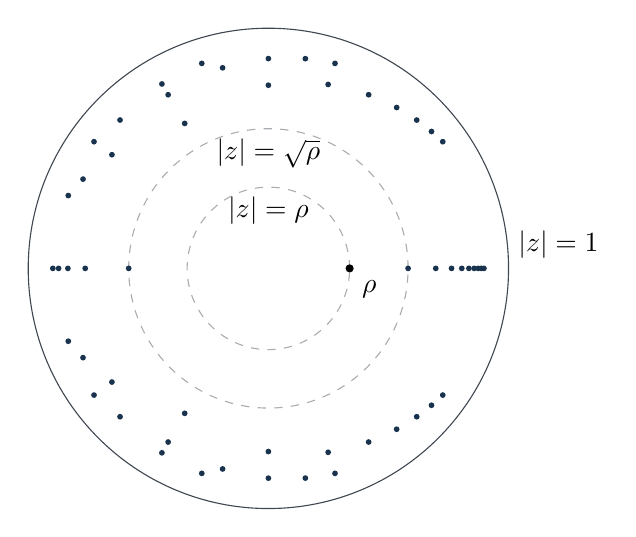
\begin{tikzpicture}[scale=3.05]
  \draw[darkgray,thin] (0,0) circle (1);
  \draw[darkgray!45,thin,dashed] (0,0) circle ({0.3383218569});
  \draw[darkgray!45,thin,dashed] (0,0) circle ({sqrt(0.3383218569)});
  \foreach \m in {1,...,10}{
    \pgfmathsetmacro{\rad}{pow(0.3383218569,1/\m)}
    \foreach \j in {0,...,9}{
      \ifnum\j<\m
        \pgfmathsetmacro{\ang}{360*\j/\m}
        \fill[deepblue] (\ang:\rad) circle (0.012);
      \fi
    }
  }
  \fill[black] ({0.3383218569},0) circle (0.017)
    node[below right=1pt] {$\rho$};
  \node[above right] at (0:1) {$|z|=1$};
  \node[below] at (90:{sqrt(0.3383218569)}) {$|z|=\sqrt\rho$};
  \node[below] at (90:{0.3383218569}) {$|z|=\rho$};
\end{tikzpicture}
\caption{The first ten root-lift layers
$z^m=\rho$.  These are a structural skeleton of the analytically continued
singularity set and accumulate at the natural boundary.}
\label{fig:singularity-skeleton}
\end{figure}

\subsection{The first explicit non-dominant sector}

The negative point
\begin{equation}
 \sigma_-=-\sqrt\rho
 =-0.581654413633394253810057781645\ldots
 \label{eq:sigma-minus}
\end{equation}
is accessible along the negative real axis.  Only the $k=2$ term in $R(z)$
reaches the dominant singularity directly.  With
$X_-=1-z/\sigma_-$,
\[
 1-\frac{z^2}{\rho}=1-(1-X_-)^2=2X_--X_-^2.
\]
Therefore the leading fractional coefficient in $R$ is $t_1/\sqrt2$.
The regular Cayley outer map gives
\begin{equation}
 \tau_{-,1/2}
 =\frac{T_-}{1-T_-}\frac{t_1}{\sqrt2},
 \qquad
 T_-=C(\zeta_-),
 \qquad
 \zeta_-=\sigma_-\exp\!\left(
 \frac12+\sum_{k\geq3}\frac{T(\sigma_-^k)}{k}\right).
 \label{eq:tau-minus}
\end{equation}
Numerically,
\begin{align*}
 \zeta_-&=-0.9293757352012050888501367\ldots,\\
 T_-&=-0.5410329414204534926205031\ldots,\\
 \tau_{-,1/2}&=0.3871501110302429034772067\ldots.
\end{align*}
Thus the leading formal Darboux contribution is
\begin{equation}
 \mathcal A_-(n)
 \sim -0.1092130299563101757054885\ldots\,
       (-\sqrt\rho)^{-n}n^{-3/2}
       \left(1+\BigO(n^{-1})\right).
 \label{eq:first-subdominant}
\end{equation}
Relative to the dominant leading term, it begins as
\begin{equation}
 \frac{\mathcal A_-(n)}{A\rho^{-n}n^{-3/2}}
 \sim -0.2482543049151649529915710\ldots\,
       (-\sqrt\rho)^n.
 \label{eq:first-relative}
\end{equation}
Its action is
\begin{equation}
 \Omega_-=\frac{\alpha}{2}+\ii\pi
 \quad(\mathrm{mod}\ 2\pi\ii),
 \label{eq:minus-action}
\end{equation}
which explains the alternating exponentially small scale
$(-1)^n\rho^{n/2}$ and the late-term divergence of the dominant inverse-power
series.

\section{Multiplicative reciprocal transseries}
\label{sec:reciprocal}

If ``inverse'' is intended as the reciprocal, the dominant algebraic answer
is immediate from \cref{eq:forward-normal}.  Let
\begin{equation}
 \frac1{F(u)}=1+\sum_{m\geq1}r_mu^m.
 \label{eq:reciprocal-F}
\end{equation}
Then
\begin{equation}
 \boxed{
 r_m=\sum_{k=1}^m(-1)^k\Bell_{m,k}(f_1,f_2,\ldots),
 \qquad m\geq1.}
 \label{eq:r-master}
\end{equation}
Consequently,
\begin{equation}
 \boxed{
 \frac1{a_n}
 \sim \frac1A\e^{-\alpha n}n^{3/2}
 \left(1+\sum_{m\geq1}\frac{r_m}{n^m}\right).}
 \label{eq:reciprocal-asymptotic}
\end{equation}
The first coefficients are
\begin{align*}
 r_1&=-0.10040348009640143476\ldots,&
 r_2&=-0.49385345628683505404\ldots,\\
 r_3&=-1.8721035437371763481\ldots,&
 r_4&=-9.8824812214415511709\ldots,\\
 r_5&=-69.510824913364618832\ldots,&
 r_6&=-616.91686459784338163\ldots.
\end{align*}

For the full multisector reciprocal, write
$a_n=M_n(1+E_n)$, where $M_n$ is the dominant all-orders sector and $E_n$ is
the sum of relative exponential sectors.  Then
\begin{equation}
 \frac1{a_n}=\frac1{M_n}\sum_{q\geq0}(-E_n)^q.
 \label{eq:reciprocal-multisector}
\end{equation}
Products generate all additive combinations of actions
$\Omega_{\sigma_1}+\cdots+\Omega_{\sigma_q}$, with coefficients obtained by
the same generalized Bell convolution \cref{eq:generalized-bell}.

\section{Asymptotic inverse of the coefficient sequence}
\label{sec:inverse}

The integer sequence has $a_1=a_2=1$ and is strictly increasing thereafter.
For large $y$, one may define the generalized inverse
\begin{equation}
 N(y)=\min\{n\geq2:a_n\geq y\}.
 \label{eq:integer-inverse}
\end{equation}
An asymptotic series describes a smooth inverse $x(y)$; the discrete answer is
obtained by rounding and can never be resolved more accurately than one unit
without using the exact sequence.  We invert the formal interpolation
obtained from \cref{eq:forward-normal}.

\subsection{Exact Lambert core}

First ignore $F(1/x)$ and solve
\begin{equation}
 y=A\e^{\alpha x}x^{-p},\qquad p=\frac32.
 \label{eq:leading-model}
\end{equation}
Taking the $p$th root and rearranging gives
\[
 -\frac{\alpha x}{p}
 \exp\!\left(-\frac{\alpha x}{p}\right)
 =-\frac{\alpha}{p}\left(\frac{A}{y}\right)^{1/p}.
\]
The large positive solution requires the lower real branch:
\begin{equation}
 \boxed{
 X(y)=-\frac{p}{\alpha}
 W_{-1}\!\left(-\frac{\alpha}{p}
                 \left(\frac{A}{y}\right)^{1/p}\right).}
 \label{eq:Lambert-core}
\end{equation}
This exact normalization absorbs all iterated logarithms caused by the factor
$x^{-p}$.

\subsection{All algebraic corrections by parameterized Lagrange inversion}

Write
\begin{equation}
 G(u)=\log F(u)=\sum_{m\geq1}g_mu^m.
 \label{eq:G-logF}
\end{equation}
By \cref{eq:bell-log},
\begin{equation}
 \boxed{
 g_m=\sum_{k=1}^m\frac{(-1)^{k-1}}{k}
 \Bell_{m,k}(f_1,f_2,\ldots).}
 \label{eq:g-master}
\end{equation}
Seek $x=X+\delta$ and put $u=1/X$.  Since $X$ solves the leading model,
substitution into the logarithm of \cref{eq:forward-normal} yields exactly
\begin{equation}
 \alpha\delta-p\log(1+u\delta)
 +G\!\left(\frac{u}{1+u\delta}\right)=0.
 \label{eq:delta-equation}
\end{equation}
Equivalently,
\begin{equation}
 \delta=\Phi(u,\delta),
 \qquad
 \Phi(u,v)=\frac p\alpha\log(1+uv)
 -\frac1\alpha G\!\left(\frac{u}{1+uv}\right).
 \label{eq:Phi}
\end{equation}
There is a unique formal solution $\delta(u)\in u\R[[u]]$.

\begin{theorem}[General coefficient formula for the inverse]
\label{thm:inverse-coefficients}
The complete algebraic inverse expansion is
\begin{equation}
 \boxed{
 x(y)\sim X(y)+\sum_{m\geq1}\frac{d_m}{X(y)^m},}
 \label{eq:inverse-X}
\end{equation}
where
\begin{equation}
 \boxed{
 d_m=\sum_{k=1}^m\frac1k
 [u^m v^{k-1}]\,\Phi(u,v)^k.}
 \label{eq:d-master}
\end{equation}
The function $\Phi$ is given by \cref{eq:Phi}, and its coefficients are
finite Bell-polynomial expressions in $f_1,\ldots,f_m$.
\end{theorem}

\begin{proof}
Treat $u$ as a parameter in the formal fixed-point equation
$v=\Phi(u,v)$.  The Lagrange--B\"urmann formula gives
\[
 \delta(u)=\sum_{k\geq1}\frac1k[v^{k-1}]\Phi(u,v)^k.
\]
Because $\Phi(u,v)=\BigO(u)$, only $k\leq m$ can contribute to $[u^m]$,
which gives \cref{eq:d-master}.  Substitution into
\cref{eq:delta-equation} proves formal inversion order by order.
\end{proof}

The first symbolic coefficients are
\begin{align}
 d_1&=-\frac{g_1}{\alpha},
 \label{eq:d1}\\
 d_2&=-\frac{\alpha g_2+pg_1}{\alpha^2},
 \label{eq:d2}\\
 d_3&=-\frac{\alpha^2g_3+\alpha g_1^2+\alpha pg_2+p^2g_1}
 {\alpha^3},
 \label{eq:d3}\\
 d_4&=-\frac{2\alpha^3g_4+6\alpha^2g_1g_2
 +2\alpha^2pg_3+5\alpha p g_1^2+2\alpha p^2g_2+2p^3g_1}
 {2\alpha^4}.
 \label{eq:d4}
\end{align}
For the Butcher tree sequence,
\begin{align*}
 g_1&=0.10040348009640143476\ldots,&
 g_2&=0.49889388569456929357\ldots,\\
 g_3&=1.9220255338418218216\ldots,&
 g_4&=10.197396423373768871\ldots,
\end{align*}
and
\begin{align*}
 d_1&=-0.092643853525613129842\ldots,&
 d_2&=-0.58856303993134726281\ldots,\\
 d_3&=-2.5966801674075310212\ldots,&
 d_4&=-13.149053399967065685\ldots,\\
 d_5&=-85.498701514625566522\ldots,&
 d_6&=-711.26291483294656090\ldots,\\
 d_7&=-7306.7882702849672566\ldots,&
 d_8&=-89561.760882637248600\ldots.
\end{align*}
As with the forward coefficients, this series is asymptotic and should be
truncated near its least term.

\subsection{Polynomial--logarithmic form and Lambert polynomials}
\label{subsec:polylog-inverse}

To express the inverse without an unevaluated Lambert function, define
\begin{equation}
 \varepsilon=\frac\alpha p\left(\frac Ay\right)^{1/p},
 \qquad
 S=\log\frac1\varepsilon
 =\frac1p\log\frac yA+\log\frac p\alpha,
 \qquad
 L=\log S.
 \label{eq:S-L}
\end{equation}
The lower branch has the complete expansion
\begin{equation}
 W_{-1}(-\varepsilon)
 =-S-L+\sum_{n\geq1}\frac{(-1)^nP_n(L)}{S^n}.
 \label{eq:Wminus-expansion}
\end{equation}
The Lambert polynomials admit either of the equivalent general formulas
\begin{align}
 P_n(u)
 &=\frac{(-1)^{n+1}}{(n+1)!}
   \left(\prod_{j=0}^{n-1}(D_u-j)\right)u^{n+1},
 \label{eq:P-operator}\\
 &=(-1)^{n+1}\sum_{k=0}^n
   \frac{s(n,k)}{(n+1-k)!}u^{n+1-k},
 \label{eq:P-stirling}
\end{align}
where $s(n,k)$ are signed Stirling numbers of the first kind.  In particular,
\begin{align*}
 P_1(u)&=u,\\
 P_2(u)&=\frac{u(u-2)}2,\\
 P_3(u)&=\frac{u(2u^2-9u+6)}6,\\
 P_4(u)&=\frac{u(3u^3-22u^2+36u-12)}{12}.
\end{align*}

Set
\begin{equation}
 V(v,L)=1+Lv-\sum_{n\geq1}(-1)^nP_n(L)v^{n+1}.
 \label{eq:V}
\end{equation}
Then $X=(p/\alpha)S V(S^{-1},L)$.  Substituting this into
\cref{eq:inverse-X} yields
\begin{equation}
 x(y)\sim\frac p\alpha(S+L)+\sum_{m\geq1}\frac{H_m(L)}{S^m}.
 \label{eq:polylog-inverse}
\end{equation}

\begin{theorem}[General polynomial--log coefficient]
\label{thm:H-coefficients}
For every $m\geq1$,
\begin{equation}
 \boxed{
 H_m(L)=-\frac p\alpha(-1)^mP_m(L)
 +\sum_{j=1}^m d_j\left(\frac\alpha p\right)^j
 [v^{m-j}]V(v,L)^{-j}.}
 \label{eq:H-master}
\end{equation}
Thus $H_m$ is an explicitly computable polynomial of degree $m$, and
\cref{eq:H-master} together with \cref{eq:d-master,eq:P-stirling} is a closed
formula for every block of the inverse logarithmic transseries.
\end{theorem}

The first two blocks simplify to
\begin{align}
 H_1(L)
 &=\frac p\alpha L-\frac{g_1}{p},
 \label{eq:H1}\\
 H_2(L)
 &=-\frac p{2\alpha}L^2
   +\left(\frac p\alpha+\frac{g_1}{p}\right)L
   -\frac{g_1}{p}-\frac{\alpha g_2}{p^2}.
 \label{eq:H2}
\end{align}
The hierarchy has the canonical form
\[
 x(y)=\frac1\alpha\log y
      +\frac p\alpha\log\log y
      +\text{constant}
      +\sum_{m\geq1}
        \frac{\text{polynomial in }\log\log y}
             {(\log y)^m},
\]
but \cref{eq:Lambert-core,eq:inverse-X} is numerically more stable because it
resums all Lambert-generated log--log terms.

\section{Exponential sectors under inversion}
\label{sec:inverse-exponential}

The inverse of the full forward transseries contains more than the algebraic
corrections in \cref{eq:inverse-X}.  Write a continuous interpolation as
\begin{equation}
 a(x)=M(x)(1+E(x)),
 \label{eq:M-E}
\end{equation}
where $M$ is the complete dominant sector and $E$ is the sum of relative
exponential sectors.  Let $x_0(y)$ be the formal inverse of $M$, given by
\cref{eq:inverse-X}, and put $x=x_0+\eta$.  Define
\begin{equation}
 Q_x(v)=\frac{\log M(x+v)-\log M(x)}{v},
 \qquad Q_x(0)=(\log M)'(x).
 \label{eq:Qx}
\end{equation}
The exact correction equation is
\begin{equation}
 \eta=\Psi_x(\eta),
 \qquad
 \Psi_x(v)=-\frac{\log(1+E(x+v))}{Q_x(v)}.
 \label{eq:Psi-exponential}
\end{equation}
A second Lagrange inversion gives
\begin{equation}
 \boxed{
 \eta(x)=\sum_{k\geq1}\frac1k[v^{k-1}]\Psi_x(v)^k.}
 \label{eq:eta-master}
\end{equation}
This single formula generates every one-sector and multi-sector correction,
including all additive combinations of actions.  Its linearization is
\begin{equation}
 \eta(x)=-\frac{E(x)}{(\log M)'(x)}+\BigO(E(x)^2)
       \sim-\frac{E(x)}\alpha.
 \label{eq:eta-leading}
\end{equation}

Suppose a forward relative sector has the form
\begin{equation}
 E_\sigma(x)=\e^{-\Omega_\sigma x}x^{\nu_\sigma}
 \mathcal F_\sigma(1/x).
 \label{eq:E-sigma}
\end{equation}
Using $y\sim A\e^{\alpha x}x^{-p}$,
\begin{equation}
 \e^{-\Omega_\sigma x}
 \sim \left(\frac yA\right)^{-\Omega_\sigma/\alpha}
 x^{-p\Omega_\sigma/\alpha}.
 \label{eq:action-map}
\end{equation}
Thus an exponentially small term in the index becomes a generally complex
power of $y$ multiplied by powers of $\log y$.  Conjugate actions combine to
produce log-periodic oscillations in the inverse variable.

For the first alternating action \cref{eq:minus-action},
\begin{equation}
 \frac{\Omega_-}{\alpha}=\frac12+\ii\frac\pi\alpha,
 \label{eq:minus-inverse-power}
\end{equation}
so the inverse has corrections whose envelope is approximately
$y^{-1/2}(\log y)^{-3/4}$ and whose phase is periodic in $\log y$ up to lower
logarithmic corrections.  Formula \cref{eq:eta-master} supplies all
coefficients once a Stokes prescription for the forward sector is fixed.

\section{Numerical validation}
\label{sec:numerics}

All numbers in this section were computed from the exact recurrence
\cref{eq:recurrence}, the scalar equation \cref{eq:rho-equation}, and the
coefficient formulas above using high-precision arithmetic.  No fit to the
sequence was used.

\subsection{Forward expansion}

Let $A_M(n)$ denote \cref{eq:forward-asymptotic} truncated after
$\kappa_M/n^M$.  Table \ref{tab:forward-errors} reports the signed relative
error $(A_M(n)-a_n)/a_n$.  The improvement is characteristic of an asymptotic
series: for fixed $n$ the error first falls rapidly, then eventually rises if
the series is over-truncated.

\begin{table}[htbp]
\centering
\caption{Signed relative error of the forward approximation.}
\label{tab:forward-errors}
\scriptsize
\setlength{\tabcolsep}{4.2pt}
\begin{tabular}{rcccccc}
\toprule
$n$ & $M=0$ & $M=2$ & $M=4$ & $M=6$ & $M=8$ & $M=10$\\
\midrule
10  & $-1.52\,10^{-2}$ & $-3.49\,10^{-4}$ & $ 2.63\,10^{-3}$ & $ 3.99\,10^{-3}$ & $ 5.52\,10^{-3}$ & $ 8.77\,10^{-3}$\\
20  & $-6.58\,10^{-3}$ & $-3.42\,10^{-4}$ & $-3.18\,10^{-5}$ & $ 1.04\,10^{-6}$ & $ 9.73\,10^{-6}$ & $ 1.41\,10^{-5}$\\
50  & $-2.22\,10^{-3}$ & $-1.77\,10^{-5}$ & $-2.88\,10^{-7}$ & $-1.20\,10^{-8}$ & $-9.84\,10^{-10}$ & $-1.36\,10^{-10}$\\
100 & $-1.06\,10^{-3}$ & $-2.08\,10^{-6}$ & $-8.06\,10^{-9}$ & $-7.88\,10^{-11}$ & $-1.50\,10^{-12}$ & $-4.73\,10^{-14}$\\
200 & $-5.15\,10^{-4}$ & $-2.53\,10^{-7}$ & $-2.40\,10^{-10}$ & $-5.73\,10^{-13}$ & $-2.66\,10^{-15}$ & $-2.04\,10^{-17}$\\
500 & $-2.03\,10^{-4}$ & $-1.59\,10^{-8}$ & $-2.39\,10^{-12}$ & $-9.02\,10^{-16}$ & $-6.62\,10^{-19}$ & $-8.01\,10^{-22}$\\
\bottomrule
\end{tabular}
\end{table}

\subsection{Inverse expansion}

For $y=a_n$, the exact continuous inverse should return $n$.  Let $X$ be the
Lambert core \cref{eq:Lambert-core}, and let
$x_M=X+\sum_{j=1}^Md_jX^{-j}$.  Table \ref{tab:inverse-errors} gives
$x_M(a_n)-n$.

\begin{table}[htbp]
\centering
\caption{Absolute index error of the Lambert-normalized inverse.}
\label{tab:inverse-errors}
\scriptsize
\setlength{\tabcolsep}{4.6pt}
\begin{tabular}{rcccccc}
\toprule
$n$ & core $X$ & $M=1$ & $M=2$ & $M=4$ & $M=6$ & $M=8$\\
\midrule
10  & $ 1.64\,10^{-2}$ & $ 7.15\,10^{-3}$ & $ 1.29\,10^{-3}$ & $-2.61\,10^{-3}$ & $-4.16\,10^{-3}$ & $-5.76\,10^{-3}$\\
20  & $ 6.55\,10^{-3}$ & $ 1.91\,10^{-3}$ & $ 4.44\,10^{-4}$ & $ 3.76\,10^{-5}$ & $-2.02\,10^{-7}$ & $-9.39\,10^{-6}$\\
50  & $ 2.11\,10^{-3}$ & $ 2.59\,10^{-4}$ & $ 2.32\,10^{-5}$ & $ 3.32\,10^{-7}$ & $ 1.26\,10^{-8}$ & $ 9.98\,10^{-10}$\\
100 & $ 9.88\,10^{-4}$ & $ 6.16\,10^{-5}$ & $ 2.74\,10^{-6}$ & $ 9.34\,10^{-9}$ & $ 8.35\,10^{-11}$ & $ 1.53\,10^{-12}$\\
200 & $ 4.78\,10^{-4}$ & $ 1.50\,10^{-5}$ & $ 3.33\,10^{-7}$ & $ 2.79\,10^{-10}$ & $ 6.09\,10^{-13}$ & $ 2.71\,10^{-15}$\\
500 & $ 1.88\,10^{-4}$ & $ 2.38\,10^{-6}$ & $ 2.10\,10^{-8}$ & $ 2.78\,10^{-12}$ & $ 9.59\,10^{-16}$ & $ 6.75\,10^{-19}$\\
\bottomrule
\end{tabular}
\end{table}

The inverse error mirrors the forward error because local inversion divides a
relative forward perturbation by approximately $(\log a)'=\alpha$.
For practical inversion at moderate size, one should truncate near the least
term and then round to the nearest admissible integer, checking adjacent
values with the exact recurrence if a certified discrete answer is required.

\section{Other inverse notions}
\label{sec:other-inverses}

\subsection{The formal compositional inverse of the OGF}

Because $T(z)=z+\BigO(z^2)$, it has a formal inverse
\begin{equation}
 Z(w)=T^{\invcomp}(w)=w-w^2+w^4-w^5+w^6-4w^7+11w^8-\cdots.
 \label{eq:formal-ogf-inverse}
\end{equation}
Lagrange inversion gives the exact coefficient formula
\begin{equation}
 \boxed{
 [w^n]Z(w)=\frac1n[z^{n-1}]
 \left(\frac z{T(z)}\right)^n
 =\frac1n[z^{n-1}]
 \exp\!\left(-n\sum_{k\geq1}\frac{T(z^k)}{k}\right).}
 \label{eq:ogf-inverse-lagrange}
\end{equation}
Together with \cref{eq:bell-exp}, this is an explicit finite Bell-polynomial
formula in $a_1,\ldots,a_{n-1}$.

Near the dominant value $w=1$, the inverse branch is actually analytic in
$(1-w)$ because it resolves the square root.  From
$T=\zeta\e^T$,
\begin{equation}
 Z(w)=\zeta^{\invcomp}(w\e^{-w})
 \label{eq:inverse-near-one}
\end{equation}
on the local branch through $Z(1)=\rho$.  Since
$w\e^{-w}-\e^{-1}$ begins quadratically at $w=1$, the local expansion of $Z$
has no linear term there.  This formal inverse is conceptually different from
the large-$y$ index inverse developed in \cref{sec:inverse}.

\subsection{Inverse branches of the Cayley factorization}

Equation \cref{eq:inverse-near-one} is also useful for local coefficient
calculus.  If
\begin{equation}
 \zeta(\rho+x)-\e^{-1}=x\varphi(x),
 \qquad \varphi(0)=\zeta'(\rho)\neq0,
\end{equation}
then
\begin{equation}
 [v^m]\bigl(\zeta^{\invcomp}(\e^{-1}+v)-\rho\bigr)
 =\frac1m[x^{m-1}]\varphi(x)^{-m}.
 \label{eq:zeta-local-inverse}
\end{equation}
Composing with
\[
 (1-s)\e^{-(1-s)}-\e^{-1}
 =-\e^{-1}\sum_{m\geq2}\frac{m-1}{m!}s^m
\]
gives every Taylor coefficient of $Z(1-s)$ by another finite ordinary-Bell
convolution.

\section{Reproducible coefficient pipeline}
\label{sec:pipeline}

The following pipeline produces the forward, reciprocal, and inverse
coefficients to any prescribed finite order.

\begin{algorithm}[Dominant and inverse coefficients to order $M$]
\label{alg:pipeline}
\begin{enumerate}
\item Compute sufficiently many exact $a_n$ using \cref{eq:bj,eq:recurrence}.
\item Solve \cref{eq:rho-equation} for $\rho$ at the desired precision.
\item For $1\leq m\leq M+1$, compute $\ell_m$ from
      \cref{eq:ell-tree-numbers}, then $h_m$ from \cref{eq:hm-bell}.
\item Compute $c_r$ from \cref{eq:c-master} and $t_r$ from
      \cref{eq:t-master} through $r=2M+1$.
\item Compute $\gamma_j(j'+1/2)$ from
      \cref{eq:eta-beta,eq:gamma-beta}, then $\kappa_m$ from
      \cref{eq:kappa-master}.
\item Normalize $f_m=\kappa_m/\kappa_0$.  Obtain reciprocal coefficients
      $r_m$ from \cref{eq:r-master}.
\item Obtain $g_m$ from \cref{eq:g-master} and inverse coefficients $d_m$
      from \cref{eq:d-master}.  If a pure log--log form is needed, generate
      $P_m$ using \cref{eq:P-stirling} and $H_m$ using
      \cref{eq:H-master}.
\item For exponentially small sectors, apply \cref{alg:all-sectors} in
      increasing modulus and transfer each local germ using
      \cref{eq:sector-transfer}.  Invert the resulting transseries with
      \cref{eq:eta-master}.
\end{enumerate}
\end{algorithm}

At fixed $M$, every Bell sum is finite.  The only infinite numerical sums are
those in \cref{eq:rho-equation,eq:ell-tree-numbers}; they converge
gometrically because their arguments are at most $\rho^2$.  Consequently,
high-order coefficients can be generated with controlled arbitrary-precision
arithmetic without numerical differentiation at a singular point.

\section{Conclusions}

The P\'olya functional equation becomes particularly transparent after the
factorization
\[
 T=C\circ\zeta,
 \qquad C(u)=-W_0(-u).
\]
The universal part is governed by one Lagrange coefficient
$[v^{r-1}]A(v)^{-r/2}$; the problem-specific part is governed by ordinary
Bell composition; and coefficient transfer is governed by Bernoulli
polynomials in the gamma-ratio expansion.  These three layers lead to the
closed master formula \cref{eq:kappa-master} for every algebraic coefficient
of A000081.

The same structure makes inversion systematic.  The exponential--power core
is inverted exactly with $W_{-1}$, the remaining algebraic corrections are a
single parameterized Lagrange series \cref{eq:d-master}, and the complete
polynomial--logarithmic blocks follow from \cref{eq:H-master}.  More distant
singularities produce exponentially small forward sectors and complex-power,
log-periodic inverse sectors; their coefficients are generated recursively by
the generalized Bell calculus of \cref{sec:global-transseries}.

The natural boundary prevents the global transseries from collapsing to a
finite list of exponentials.  It does not prevent an all-orders description:
for each finite continuation domain, the local-sector recursion and transfer
formula give the complete expansion associated with every singularity
encountered there, and these finite descriptions form a coherent directed
system as the domain approaches the unit circle.

\appendix

\section{Additional low-order inverse coefficients}

For reference, the fifth inverse coefficient is
\begin{align*}
 d_5=-\frac1{2\alpha^5}\Bigl(&2\alpha^4g_5
 +8\alpha^3g_1g_3+4\alpha^3g_2^2+2\alpha^3pg_4
 +4\alpha^2g_1^3\\
 &+14\alpha^2p g_1g_2+2\alpha^2p^2g_3
 +9\alpha p^2g_1^2+2\alpha p^3g_2+2p^4g_1\Bigr).
\end{align*}
Higher expressions grow rapidly in size; \cref{eq:d-master} is both shorter
and less error-prone.

\section{Why analytic local terms do not enter the dominant sector}

A nonnegative integer power $(1-z/\rho)^m$ is a polynomial and has no
coefficients past degree $m$.  More generally, the entire analytic germ at
$z=\rho$ can be continued through $\rho$ and therefore contributes on scales
determined by its next singularities, not on the algebraic
$\rho^{-n}n^{-j}$ scale.  This is why only the odd Puiseux coefficients
$t_{2j+1}$ appear in \cref{eq:kappa-master}.  In an exponentially completed
analysis, the analytic germ is not discarded; it reappears through the
sector recursion at more distant singularities.

\section{References}

\begin{thebibliography}{99}

\bibitem{BellBurrisYeats2006}
J.~P. Bell, S.~N. Burris, and K.~A. Yeats,
\newblock Counting rooted trees: the universal law
$t(n)\sim C\rho^{-n}n^{-3/2}$,
\newblock \emph{Electronic Journal of Combinatorics} 13 (2006), R63,
\newblock \url{https://doi.org/10.37236/1089}.

\bibitem{Butcher2016}
J.~C. Butcher,
\newblock \emph{Numerical Methods for Ordinary Differential Equations},
third edition,
\newblock Wiley, 2016.

\bibitem{Comtet1974}
L.~Comtet,
\newblock \emph{Advanced Combinatorics: The Art of Finite and Infinite
Expansions},
\newblock Reidel, 1974.

\bibitem{CorlessEtAl1996}
R.~M. Corless, G.~H. Gonnet, D.~E.~G. Hare, D.~J. Jeffrey, and D.~E. Knuth,
\newblock On the Lambert $W$ function,
\newblock \emph{Advances in Computational Mathematics} 5 (1996), 329--359,
\newblock \url{https://doi.org/10.1007/BF02124750}.

\bibitem{DrmotaGittenberger2010}
M.~Drmota and B.~Gittenberger,
\newblock The shape of unlabeled rooted random trees,
\newblock \emph{European Journal of Combinatorics} 31 (2010), 2028--2063,
\newblock \url{https://arxiv.org/abs/1003.1322}.

\bibitem{FlajoletSedgewick2009}
P.~Flajolet and R.~Sedgewick,
\newblock \emph{Analytic Combinatorics},
\newblock Cambridge University Press, 2009,
\newblock \url{https://doi.org/10.1017/CBO9780511801655}.

\bibitem{Genitrini2016}
A.~Genitrini,
\newblock Full asymptotic expansion for P\'olya structures,
\newblock in \emph{Proceedings of the 27th International Conference on
Probabilistic, Combinatorial and Asymptotic Methods for the Analysis of
Algorithms}, 2016,
\newblock \url{https://arxiv.org/abs/1605.00837}.

\bibitem{HararyRobinsonSchwenk1975}
F.~Harary, R.~W. Robinson, and A.~J. Schwenk,
\newblock Twenty-step algorithm for determining the asymptotic number of
trees of various species,
\newblock \emph{Journal of the Australian Mathematical Society, Series A}
20 (1975), 483--503.

\bibitem{Knuth1997}
D.~E. Knuth,
\newblock \emph{The Art of Computer Programming, Volume 1: Fundamental
Algorithms}, third edition,
\newblock Addison--Wesley, 1997.

\bibitem{OEISA000081}
OEIS Foundation,
\newblock A000081: number of unlabeled rooted trees with $n$ nodes,
\newblock \url{https://oeis.org/A000081}, accessed September 3, 2026.

\bibitem{Otter1948}
R.~Otter,
\newblock The number of trees,
\newblock \emph{Annals of Mathematics} 49 (1948), 583--599,
\newblock \url{https://doi.org/10.2307/1969046}.

\bibitem{Polya1937}
G.~P\'olya,
\newblock Kombinatorische Anzahlbestimmungen f\"ur Gruppen, Graphen und
chemische Verbindungen,
\newblock \emph{Acta Mathematica} 68 (1937), 145--254,
\newblock \url{https://doi.org/10.1007/BF02546665}.

\bibitem{ProveItCCC}
V.~Reshetnikov,
\newblock Combinatorial Coefficient Calculus,
\newblock ProveIt repository,
\newblock \url{https://github.com/VladimirReshetnikov/ProveIt/tree/main/Analysis/FabiusFunction/docs/semi-formalized-research-frontiers/drafts/combinatorial-coefficient-calculus/Combinatorial_Coefficient_Calculus},
accessed September 3, 2026.

\bibitem{ProveItTransseries}
V.~Reshetnikov,
\newblock Series and transseries research drafts,
\newblock ProveIt repository,
\newblock \url{https://github.com/VladimirReshetnikov/ProveIt/tree/main/Analysis/FabiusFunction/docs/semi-formalized-research-frontiers/drafts/series-and-transseries},
accessed September 3, 2026.

\end{thebibliography}

\end{document}
